% Бүлэг 3

\section{Зохиомж} 
	
	\subsection{Системийн үйл ажиллагааны тухай}
	\begin{flushleft}
	Багш гар утаснаасаа оюутны бөглөсөн шабломыг камераар даран илгээснээр тухайн дугаартай оюутны дүн өс-нд хадгалагдана. Тухайн шалгалтын оюутнуудын жагсаалтан тухайн оюутны дүн багшд харагдах болно.
	\end{flushleft}
	\subsection{Юзкейс диаграм}
	\begin{flushleft}
	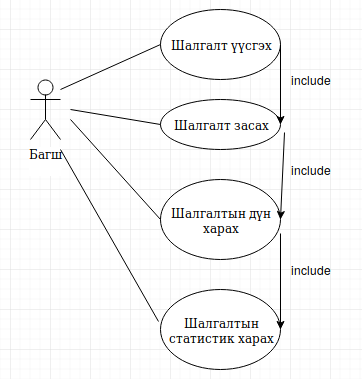
\includegraphics[width=15cm,height=6cm, scale=0.5]{Figures/cusecase.png}
	\hspace*{0pt}\hfill Багш шаблом урьчилан бэлдэж шалгалт авах үйл ажиллагааны диаграм.
	\newline
	\newline
	\end{flushleft}
	
	\subsection{Үйл ажиллагааны диаграм}
	\begin{flushleft}
	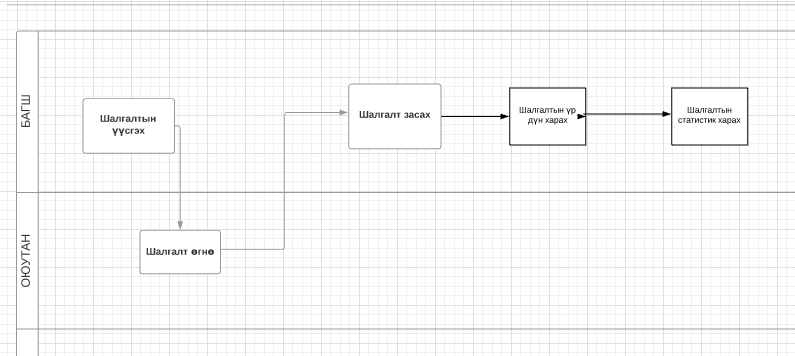
\includegraphics[width=15cm,height=6cm, scale=0.5]{Figures/cactivity.png}
	\hspace*{0pt}\hfill Багш шаблом урьчилан бэлдэж шалгалт авах үйл ажиллагааны диаграм.
	\newline
	\newline
	\end{flushleft}
	
	\subsection{Класс диаграм}
	\subsection{Дарааллын диаграм}

	\subsection{Бүлгийн дүгнэлт}
	